\chapter{DNA: een universeel erfelijk molecuul}\label{ch:g10:universal-dna}

In een verduisterd laboratorium, onder een blauwe lamp, gloeit een van
twee witte muizen groen op van neus tot staart. Zij draagt, in elk van
haar \omterm{def:g10:cells-common-unit:cell}{cellen}, één enkel \omterm{def:g10:universal-dna:gene}{gen} dat afkomstig is van een kwal die in de
Stille Oceaan oplicht --- en de \omterm{def:g10:cells-common-unit:cell}{cellen} van de muis lezen dat kwallengen
precies zoals de \omterm{def:g10:cells-common-unit:cell}{cellen} van de kwal dat doen. De proef lukt omdat elk
levend wezen zijn \omterm{def:g10:universal-dna:gene}{genen} in hetzelfde molecuul schrijft, met dezelfde
vier letters, en ze volgens dezelfde regels leest. Dit hoofdstuk gaat
over dat molecuul, het \omterm{def:g10:universal-dna:information}{DNA}: hoe het gebouwd is, wat zijn structuur
verklaart, en wat de gloeiende muis bewijst.

\section{Het erfelijk materiaal}

\begin{definition}[Genetische informatie]\label{def:g10:universal-dna:information}
De \emph{genetische informatie}\index{genetische informatie} van een \omterm{def:g10:cells-common-unit:cell}{cel}
is het geheel van instructies dat van een \omterm{def:g10:cells-common-unit:cell}{cel} op haar dochtercellen en
van ouders op nakomelingen wordt doorgegeven, en dat de kenmerken van
het organisme bepaalt en de \omterm{def:g10:chemistry-of-life:families}{eiwitten} die zijn \omterm{def:g10:cells-common-unit:cell}{cellen} kunnen maken. In
elk levend wezen wordt zij gedragen door moleculen
\emph{DNA}\index{DNA} (desoxyribonucleïnezuur), die met \omterm{def:g10:chemistry-of-life:families}{eiwitten} zijn
verpakt tot de \emph{chromosomen}\index{chromosoom} --- in de \omterm{def:g10:cells-common-unit:organelle}{celkern}
van een \omterm{def:g10:cells-common-unit:prokaryote}{eukaryote cel}, vrij in het \omterm{def:g10:cells-common-unit:cell}{cytoplasma} van een bacterie.
\end{definition}

\begin{proposition}[DNA is het molecuul van de erfelijkheid]\label{prop:g10:universal-dna:material}
Het erfelijk materiaal van een \omterm{def:g10:cells-common-unit:cell}{cel} is haar \omterm{def:g10:universal-dna:information}{DNA}, niet haar \omterm{def:g10:chemistry-of-life:families}{eiwitten} of
enig ander bestanddeel: gezuiverd \omterm{def:g10:universal-dna:information}{DNA} van de ene bacteriestam naar de
andere overbrengen, brengt de kenmerken van de eerste stam mee over.
\end{proposition}
\begin{proof}[Bewijsmateriaal]
Griffith (1928) ontdekte dat onschadelijke longontstekingsbacteriën,
gemengd met gedode \omterm{def:g10:cells-common-unit:cell}{cellen} van een dodelijke stam, dodelijk werden en dat
generaties lang bleven: iets uit de dode \omterm{def:g10:cells-common-unit:cell}{cellen} had hen
"getransformeerd". Avery, MacLeod en McCarty (1944) scheidden het
extract van de dode \omterm{def:g10:cells-common-unit:cell}{cellen} in zijn moleculenfamilies en toetsten elke
familie afzonderlijk: alleen de DNA-fractie transformeerde; het extract
behandelen met een enzym dat \omterm{def:g10:universal-dna:information}{DNA} afbreekt hief het effect op, terwijl
enzymen die \omterm{def:g10:chemistry-of-life:families}{eiwitten} of RNA afbreken dat niet deden. De transformerende
stof, en dus de drager van het erfelijke kenmerk, was \omterm{def:g10:universal-dna:information}{DNA}.
\end{proof}

\begin{example}[Waar het DNA zit]\label{ex:g10:universal-dna:where}
Een kleurstof die specifiek op \omterm{def:g10:universal-dna:information}{DNA} aanslaat, kleurt de \omterm{def:g10:cells-common-unit:organelle}{celkern} van een
wangcel en verder niets in het \omterm{def:g10:cells-common-unit:cell}{cytoplasma}; in een delende \omterm{def:g10:cells-common-unit:cell}{cel} kleurt zij
de compacte \omterm{def:g10:universal-dna:information}{chromosomen}. Een bacterie neemt de kleurstof op in een
middengebied zonder omhulsel. In beide gevallen verdubbelt de
hoeveelheid \omterm{def:g10:universal-dna:information}{DNA} vóór elke deling en wordt zij tussen de twee
dochtercellen gehalveerd --- het gedrag dat je verwacht van informatie
die moet worden gekopieerd en gedeeld.
\end{example}

\section{De bouw van het DNA}

\begin{definition}[Nucleotide]\label{def:g10:universal-dna:nucleotide}
\omterm{def:g10:universal-dna:information}{DNA} is een keten van \emph{nucleotiden}\index{nucleotide}. Elke
nucleotide bestaat uit drie delen: een fosfaatgroep, een suiker
(desoxyribose) en een van vier stikstofhoudende
\emph{basen}\index{base (DNA)}: adenine (A), thymine (T), guanine (G) en
cytosine (C). Suikers en fosfaten wisselen elkaar af en vormen de
ruggengraat van de keten; de basen steken daaruit naar buiten, één per
nucleotide. De vier nucleotiden verschillen alleen in hun base, zodat
een DNA-streng wordt beschreven door de volgorde van zijn basen,
geschreven als een rij letters: \texttt{ATGGCTTAC\dots}
\end{definition}

\begin{omfigure}
\begin{tikzpicture}[>=Stealth, font=\small]
  % left strand backbone
  \foreach \i in {0,...,5} {
    \draw[fill=gray!30] (0,{1.1*\i}) circle (0.22);           % phosphate
    \draw[fill=omDef!25] (0.9,{1.1*\i+0.15}) -- (1.35,{1.1*\i+0.45}) -- (1.35,{1.1*\i-0.15}) -- (0.9,{1.1*\i-0.45}) -- (0.55,{1.1*\i}) -- cycle; % sugar (pentagon)
    \draw (0.22,{1.1*\i}) -- (0.55,{1.1*\i});
    \draw (1.35,{1.1*\i+0.45}) -- (0,{1.1*\i+1.1-0.22});
  }
  \foreach \i in {0,...,5} {
    \draw[fill=gray!30] (7.6,{1.1*\i+0.55}) circle (0.22);
    \draw[fill=omDef!25] (6.7,{1.1*\i+0.55+0.15}) -- (6.25,{1.1*\i+0.55+0.45}) -- (6.25,{1.1*\i+0.55-0.15}) -- (6.7,{1.1*\i+0.55-0.45}) -- (7.05,{1.1*\i+0.55}) -- cycle;
    \draw (7.38,{1.1*\i+0.55}) -- (7.05,{1.1*\i+0.55});
  }
  \foreach \i in {0,...,4}
    \draw (6.25,{1.1*\i+0.55+0.45}) -- (7.6,{1.1*\i+0.55+1.1-0.22});
  % base pairs
  \foreach \i/\l/\r/\cl/\cr in {0/A/T/omThm/omMeth, 1/G/C/omProp/omDef,
      2/C/G/omDef/omProp, 3/T/A/omMeth/omThm, 4/A/T/omThm/omMeth, 5/G/C/omProp/omDef} {
    \draw[fill=\cl!40] (1.35,{1.1*\i+0.15-0.25}) rectangle (3.7,{1.1*\i+0.15+0.25});
    \node at (2.5,{1.1*\i+0.15}) {\l};
    \draw[fill=\cr!40] (3.9,{1.1*\i+0.15-0.25}) rectangle (6.25,{1.1*\i+0.15+0.25});
    \node at (5.1,{1.1*\i+0.15}) {\r};
    \draw[densely dotted, thick] (3.7,{1.1*\i+0.15}) -- (3.9,{1.1*\i+0.15});
  }
  \node[anchor=east, align=right] at (-0.4,2.9) {ruggengraat\\ van fosfaat\\ en suiker};
  \node[anchor=west, align=left] at (8.0,3.45) {tweede\\ streng};
  \node[anchor=south] at (2.5,6.5) {basen, gepaard};
  \draw[->] (0,-0.5) -- (0,-1.0) node[below] {richting van streng 1};
  \draw[->] (7.6,0.05) -- (7.6,-1.0) node[below] {streng 2, tegengesteld};
  \draw[<->, thick] (8.9,0.15) -- (8.9,1.25) node[midway, right] {\qty{0.34}{nm}};
\end{tikzpicture}

{\small De twee strengen van het \omterm{def:g10:universal-dna:information}{DNA}, plat getekend. Elke streng is een
keten van \omterm{def:g10:universal-dna:nucleotide}{nucleotiden} (fosfaat, suiker, base). De strengen lopen in
tegengestelde richting en worden bijeengehouden door basenparen: A staat
altijd tegenover T, G altijd tegenover C. Elke \qty{0.34}{nm} volgt het
volgende basenpaar.}
\end{omfigure}

\begin{proposition}[De dubbele helix]\label{prop:g10:universal-dna:helix}
Een DNA-molecuul bestaat uit twee strengen die om elkaar heen gewonden
zijn tot een rechtsdraaiende \emph{dubbele helix}\index{dubbele helix}
van ongeveer \qty{2}{nm} breed, met één winding per tien basenparen
(\qty{3.4}{nm}). De strengen lopen in tegengestelde richting en staan
met hun basen tegenover elkaar; die basen paren volgens een strenge
regel van \emph{complementariteit}\index{complementariteit}: A paart
alleen met T, G alleen met C. De volgorde van de ene streng legt daarmee
de volgorde van de andere vast.
\end{proposition}
\begin{proof}[Bewijsmateriaal]
Chargaff (1950) mat de basensamenstelling van \omterm{def:g10:universal-dna:information}{DNA} van vele soorten en
vond in elke soort evenveel A als T en evenveel G als C, terwijl de
verhouding van A+T tot G+C van soort tot soort varieerde --- een
paringsregel, geen chemisch toeval. De röntgenopnamen van DNA-vezels
door Franklin (1952) toonden het handschrift van een helix met
\qty{2}{nm} doorsnede en \qty{3.4}{nm} spoed. Watson en Crick (1953)
bouwden het enige model dat bij beide past: twee ruggengraten aan de
buitenkant, gepaarde basen aan de binnenkant, waarbij de paren A--T en
G--C even breed zijn zodat de helix regelmatig blijft.
\end{proof}

\begin{example}[De regel van Chargaff in cijfers]\label{ex:g10:universal-dna:chargaff}
Menselijk \omterm{def:g10:universal-dna:information}{DNA}: A 30.9\%, T 29.4\%, G 19.9\%, C 19.8\% --- A$\,\approx\,$T
en G$\,\approx\,$C tot op de meetnauwkeurigheid, en A+T $= 60\%$.
\emph{E.~coli}: A 24.7\%, T 23.6\%, G 26.0\%, C 25.7\%, A+T $= 48\%$.
Gist: A+T $= 64\%$. Bevat een DNA-monster 32\% A, dan voorspelt de
\omterm{prop:g10:universal-dna:helix}{complementariteit} 32\% T en $(100 - 64)/2 = 18\%$ G en evenveel C.
\end{example}

\begin{omfigure}
\begin{tikzpicture}
\begin{axis}[
  ybar, bar width=7pt,
  width=0.86\linewidth, height=5.4cm,
  axis x line=bottom, axis y line=left,
  ymin=0, ymax=40, ylabel={\% van de basen}, ylabel style={font=\small},
  symbolic x coords={mens, gist, E. coli, tarwe},
  xtick=data, tick label style={font=\small},
  enlarge x limits=0.18,
  legend style={at={(0.5,-0.2)}, anchor=north, legend columns=4,
                font=\small, draw=none},
]
\addplot[fill=omThm!50, draw=omThm] coordinates {(mens,30.9) (gist,31.3) (E. coli,24.7) (tarwe,27.3)};
\addplot[fill=omMeth!60, draw=omMeth] coordinates {(mens,29.4) (gist,32.9) (E. coli,23.6) (tarwe,27.1)};
\addplot[fill=omProp!50, draw=omProp] coordinates {(mens,19.9) (gist,18.7) (E. coli,26.0) (tarwe,22.7)};
\addplot[fill=omDef!50, draw=omDef] coordinates {(mens,19.8) (gist,17.1) (E. coli,25.7) (tarwe,22.8)};
\legend{A, T, G, C}
\end{axis}
\end{tikzpicture}

{\small Basensamenstelling van het \omterm{def:g10:universal-dna:information}{DNA} in vier typen. In elk type
zijn de staven van A en T even hoog en die van G en C ook --- het
handschrift van de basenparing --- terwijl het aandeel A+T van soort tot
soort verschilt.}
\end{omfigure}

\begin{method}[De complementaire streng schrijven]\label{met:g10:universal-dna:complement}
Schrijf, gegeven één streng, onder elke base haar partner
(A$\leftrightarrow$T, G$\leftrightarrow$C), en lees het resultaat
vervolgens in de tegengestelde richting als de afspraak van de opgave
dat verlangt. Bij \texttt{5'-ATGGCTTAC-3'} luidt de partnerstreng,
gelezen in haar eigen richting, \texttt{5'-GTAAGCCAT-3'}. Tellen: een
streng met $n_\mathrm{A}$ adenines staat tegenover een streng met
$n_\mathrm{A}$ thymines, dus geldt in het hele molecuul
$n_\mathrm{A} = n_\mathrm{T}$ en $n_\mathrm{G} = n_\mathrm{C}$.
\end{method}

\begin{proposition}[Wat de structuur verklaart]\label{prop:g10:universal-dna:explains}
Twee eigenschappen van het erfelijk materiaal volgen uit de structuur.
\begin{itemize}
  \item \emph{Informatie}: de volgorde van de basen langs een streng
        wordt door de chemie niet vastgelegd --- elke volgorde is
        mogelijk --- zodat die volgorde een boodschap kan dragen, zoals
        de volgorde van letters een tekst draagt. Een menselijke \omterm{def:g10:cells-common-unit:cell}{cel}
        bevat $\num{3.2e9}$ basenparen in elke set \omterm{def:g10:universal-dna:information}{chromosomen}.
  \item \emph{Kopiëren}: omdat elke streng de andere vastlegt, kan het
        molecuul worden verdubbeld door de strengen te scheiden en op
        elk een nieuwe partner te bouwen. Het mechanisme is het
        onderwerp van \cref{ch:g11:dna-replication}.
\end{itemize}
\end{proposition}
\admitted

\section{Genen, allelen, chromosomen}

\begin{definition}[Gen en allel]\label{def:g10:universal-dna:gene}
Een \emph{gen}\index{gen} is een stuk van een DNA-molecuul --- meestal
enkele duizenden basenparen --- waarvan de volgorde de instructies
draagt om één \omterm{def:g10:chemistry-of-life:families}{eiwit} te maken (of soms één werkzaam RNA-molecuul). Het
neemt een vaste plaats op een bepaald \omterm{def:g10:universal-dna:information}{chromosoom} in. De versies van een
gen die in enkele basen verschillen, zijn zijn
\emph{allelen}\index{allel}: dezelfde plaats, dezelfde functie, een
iets andere volgorde, en dus vaak een iets ander \omterm{def:g10:chemistry-of-life:families}{eiwit}.
\end{definition}

\begin{example}[Getallen]\label{ex:g10:universal-dna:numbers}
Het menselijk genoom --- één volledige set \omterm{def:g10:universal-dna:information}{chromosomen} --- draagt
$\num{3.2e9}$ basenparen en ongeveer $\num{20000}$ \omterm{def:g10:universal-dna:gene}{genen}; de \omterm{def:g10:universal-dna:gene}{genen}
beslaan slechts enkele procenten van de volgorde. Een \omterm{def:g10:cells-common-unit:cell}{cel} van
\emph{E.~coli} draagt één ringvormig DNA-molecuul van $\num{4.6e6}$
basenparen en ongeveer 4300 \omterm{def:g10:universal-dna:gene}{genen}. Twee niet-verwante mensen verschillen
in ruwweg één base op duizend: zo'n drie miljoen posities, de meeste
buiten \omterm{def:g10:universal-dna:gene}{genen} en zonder gevolg, enkele daarvan \omterm{def:g10:universal-dna:gene}{allelen} die een kenmerk
veranderen.
\end{example}

\begin{proposition}[Chromosomen]\label{prop:g10:universal-dna:chromosome}
Een \omterm{def:g10:universal-dna:information}{chromosoom} is één DNA-molecuul, om verpakkingseiwitten gewonden en
op zichzelf opgerold. Uitgestrekt zou het \omterm{def:g10:universal-dna:information}{DNA} van één menselijk
\omterm{def:g10:universal-dna:information}{chromosoom} \qty{1.5}{cm} tot \qty{8.5}{cm} lang zijn; de 46 \omterm{def:g10:universal-dna:information}{chromosomen}
van een \omterm{def:g10:cells-common-unit:cell}{cel} bevatten samen ongeveer \qty{2}{m} \omterm{def:g10:universal-dna:information}{DNA} in een \omterm{def:g10:cells-common-unit:organelle}{celkern} van
\qty{6}{\micro m} doorsnee. \omterm{def:g10:universal-dna:information}{Chromosomen} zijn alleen tijdens de celdeling
als afzonderlijke lichaampjes zichtbaar, wanneer ze het strakst zijn
opgerold; tussen twee delingen zijn ze afgewikkeld en vullen ze de kern
als een kluwen.
\end{proposition}
\admitted

\section{Eén molecuul voor alle levende wezens}

\begin{proposition}[Universaliteit van het DNA]\label{prop:g10:universal-dna:universal}
Alle levende wezens --- bacteriën, schimmels, planten, dieren --- dragen
hun \omterm{def:g10:universal-dna:information}{genetische informatie} als \omterm{def:g10:universal-dna:information}{DNA} dat uit dezelfde vier \omterm{def:g10:universal-dna:nucleotide}{nucleotiden} is
gebouwd, en lezen de volgorde van een \omterm{def:g10:universal-dna:gene}{gen} volgens dezelfde regels. Een
\omterm{def:g10:universal-dna:gene}{gen} dat uit de ene soort wordt gehaald en in het \omterm{def:g10:universal-dna:information}{DNA} van een andere
wordt ingebracht, wordt daardoor door de \omterm{def:g10:cells-common-unit:cell}{cellen} van de ontvanger
gelezen, die het \omterm{def:g10:chemistry-of-life:families}{eiwit} maken waarvoor het codeert:
\emph{transgenese}\index{transgenese} is mogelijk, en het transgene
organisme geeft het vreemde \omterm{def:g10:universal-dna:gene}{gen} net als elk ander aan zijn nakomelingen
door.
\end{proposition}
\begin{proof}[Bewijsmateriaal]
Het \omterm{def:g10:universal-dna:gene}{gen} voor het groen fluorescerende \omterm{def:g10:chemistry-of-life:families}{eiwit} (GFP) van de kwal
\emph{Aequorea victoria} is ingebracht in bacteriën, gist, planten,
vissen, muizen en konijnen: alle maken zij het \omterm{def:g10:chemistry-of-life:families}{eiwit} en gloeien zij
groen onder blauw licht, en het kenmerk is erfelijk. Het menselijke \omterm{def:g10:universal-dna:gene}{gen}
voor insuline, in 1978 in \emph{E.~coli} ingebracht, laat de bacterie
menselijke insuline maken, sindsdien de bron van het hormoon voor
diabetespatiënten. Er is geen soort bekend waarvan de \omterm{def:g10:universal-dna:gene}{genen} in een
andere chemie zijn geschreven.
\end{proof}

\begin{omfigure}
\begin{tikzpicture}[>=Stealth, font=\small,
  org/.style={draw, rounded corners, minimum height=1.0cm, text width=3.0cm,
              align=center},
  dna/.style={draw, fill=omDef!12, rounded corners, minimum height=0.7cm,
              text width=3.0cm, align=center, font=\small}]
  \node[org, fill=omMeth!10] (j) at (0,0) {kwal\\ (donor)};
  \node[dna] (jd) at (0,-1.6) {DNA met het\\ GFP-gen};
  \node[dna, fill=omThm!12] (g) at (5.0,-1.6) {GFP-gen\\ geïsoleerd, gekopieerd};
  \node[dna] (md) at (10.0,-1.6) {muizen-DNA +\\ GFP-gen};
  \node[org, fill=omProp!10] (m) at (10.0,0) {eicel van de muis\\ (ontvanger)};
  \node[org, fill=omMeth!10] (t) at (10.0,-3.4) {transgene muis:\\ gloeit groen};
  \draw[->] (j) -- (jd);
  \draw[->] (jd) -- node[above] {uitgeknipt} (g);
  \draw[->] (g) -- node[above] {ingebracht} (md);
  \draw[->] (m) -- (md);
  \draw[->] (md) -- node[right] {delingen} (t);
  \node[anchor=north, text width=6.5cm, align=center] at (5.0,-2.6)
    {de cellen van de muis lezen het kwallengen\\ en maken het kwalleneiwit};
\end{tikzpicture}

{\small \omterm{prop:g10:universal-dna:universal}{Transgenese}: een \omterm{def:g10:universal-dna:gene}{gen} dat uit de ene soort is geïsoleerd, wordt in
het \omterm{def:g10:universal-dna:information}{DNA} van een bevruchte eicel van een andere soort ingebracht. Elke \omterm{def:g10:cells-common-unit:cell}{cel}
van het ontstane organisme draagt het, leest het en geeft het door.}
\end{omfigure}

\begin{omfigure}
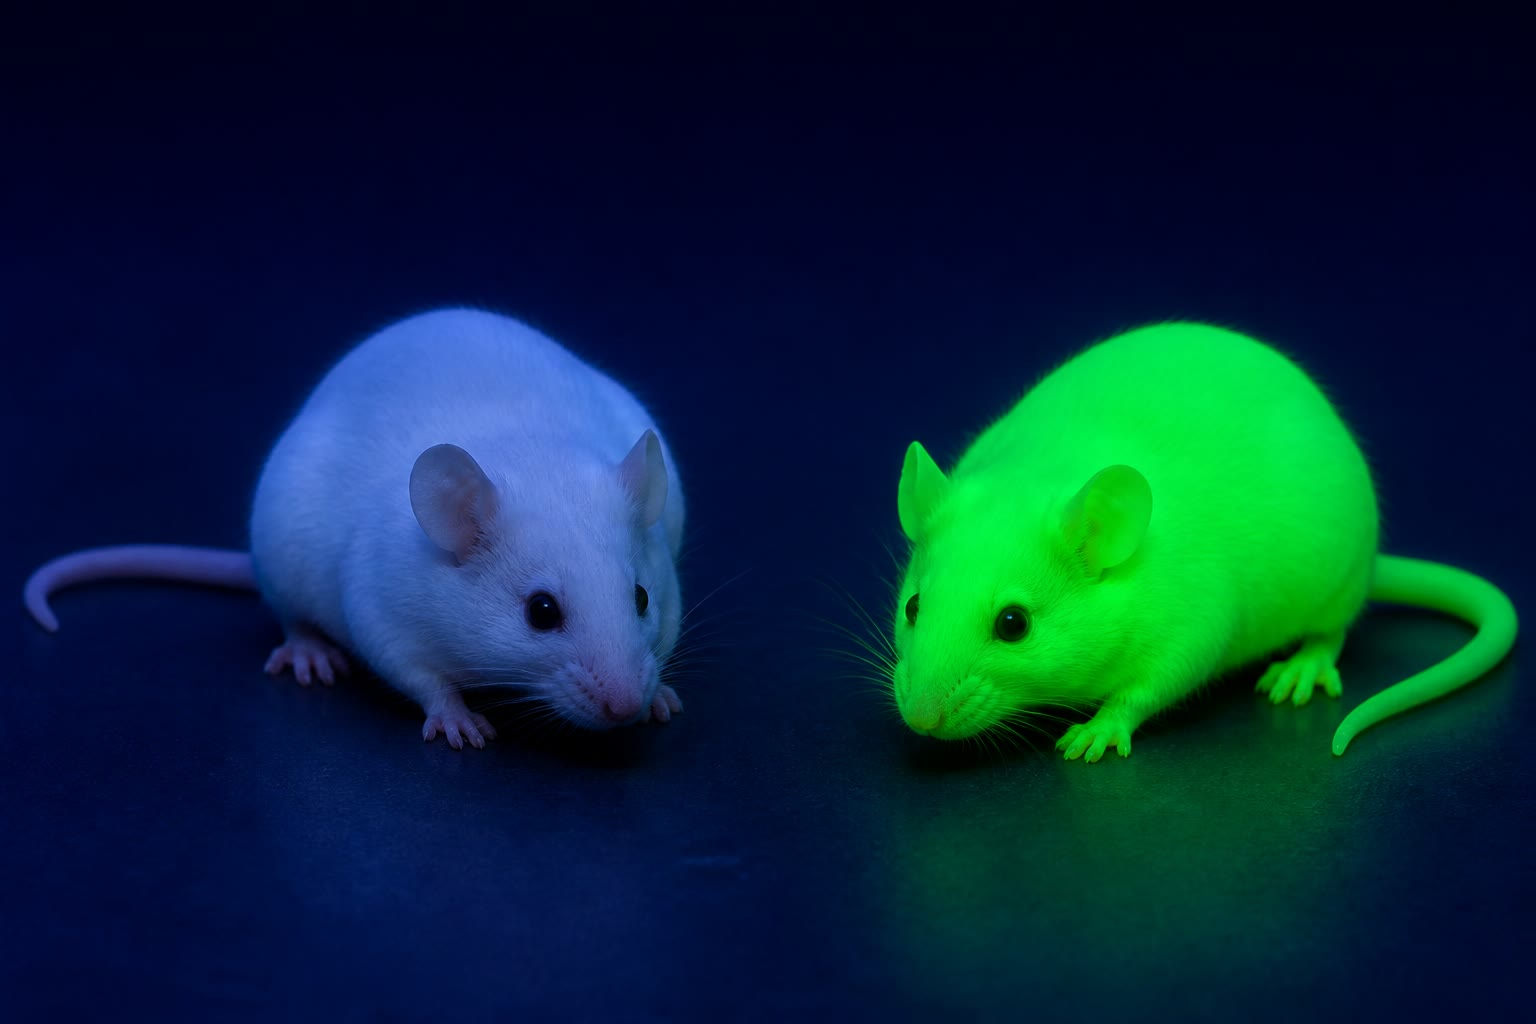
\includegraphics[width=0.62\linewidth]{images/book2/ai/g10-dna-gfp-mice.jpg}

{\small Onder blauw licht gloeit een muis die het kwallengen voor het
groen fluorescerende \omterm{def:g10:chemistry-of-life:families}{eiwit} draagt, naast een gewone muis. Hetzelfde
molecuul, dezelfde leesregels: de instructie van de kwal draait in de
muis.}
\end{omfigure}

\begin{example}[Toepassingen van transgenese]\label{ex:g10:universal-dna:uses}
Menselijke insuline en groeihormoon uit bacteriën; een \omterm{def:g10:universal-dna:gene}{gen} voor
weerstand tegen een insectenplaag ingebracht in mais of katoen; rijst
met \omterm{def:g10:universal-dna:gene}{genen} om een voorloper van vitamine A te maken; het \omterm{def:g10:universal-dna:gene}{GFP-gen} gekoppeld
aan een ander \omterm{def:g10:universal-dna:gene}{gen}, zodat de \omterm{def:g10:cells-common-unit:cell}{cellen} waarin dat \omterm{def:g10:universal-dna:gene}{gen} actief is onder de
microscoop oplichten --- die laatste toepassing, een
onderzoeksgereedschap, is verreweg de gewoonste. Elke toepassing roept
haar eigen vragen op over veiligheid en over gevolgen voor het milieu;
elke berust op hetzelfde feit, de universaliteit van het erfelijke
molecuul.
\end{example}

\begin{remark}[Eenheid en verscheidenheid op moleculair niveau]\label{rem:g10:universal-dna:unity}
De universaliteit van het \omterm{def:g10:universal-dna:information}{DNA} is het moleculaire gezicht van de eenheid
van het leven uit \cref{ch:g10:chemistry-of-life}: één chemie, één
informatiemolecuul, één leessysteem voor elk organisme op aarde, en dat
is precies wat een gemeenschappelijke oorsprong voorspelt
(\cref{ch:g10:common-ancestry}). Ook de verscheidenheid van het leven is
in datzelfde molecuul geschreven, als verschillen in volgorde: tussen
twee \omterm{def:g10:universal-dna:gene}{allelen} enkele basen, tussen twee soorten enkele procenten van het
genoom, tussen een bacterie en een mens de hele ordening van de tekst.
\end{remark}

\section{Oefeningen}

\begin{exercise}[$\star$]\label{exo:g10:universal-dna:1}
Noem de drie delen van een \omterm{def:g10:universal-dna:nucleotide}{nucleotide} en de vier basen van het \omterm{def:g10:universal-dna:information}{DNA}.
\end{exercise}

\begin{exercise}[$\star$]\label{exo:g10:universal-dna:2}
Schrijf de streng die complementair is aan \texttt{TACGGATTCA}.
\end{exercise}

\begin{exercise}[$\star$]\label{exo:g10:universal-dna:3}
Een DNA-monster bevat 21\% guanine. Geef de percentages van C, A en T.
\end{exercise}

\begin{exercise}[$\star$]\label{exo:g10:universal-dna:4}
Definieer \omterm{def:g10:universal-dna:gene}{gen} en \omterm{def:g10:universal-dna:gene}{allel} in telkens één zin, met het woord "volgorde".
\end{exercise}

\begin{exercise}[$\star$]\label{exo:g10:universal-dna:5}
Wat is een transgeen organisme? Geef twee voorbeelden uit het hoofdstuk.
\end{exercise}

\begin{exercise}[$\star\star$]\label{exo:g10:universal-dna:6}
Een \omterm{def:g10:universal-dna:gene}{gen} is 1500 basenparen lang. Wat is zijn lengte in nanometers, en
hoeveel windingen van de helix maakt het?
\end{exercise}

\begin{exercise}[$\star\star$]\label{exo:g10:universal-dna:7}
Bereken de totale lengte van het \omterm{def:g10:universal-dna:information}{DNA} in één menselijke \omterm{def:g10:cells-common-unit:cell}{cel}, gegeven
$\num{3.2e9}$ basenparen per set \omterm{def:g10:universal-dna:information}{chromosomen} en twee sets per \omterm{def:g10:cells-common-unit:cell}{cel}.
Vergelijk met de doorsnede van de \omterm{def:g10:cells-common-unit:organelle}{celkern}, \qty{6}{\micro m}.
\end{exercise}

\begin{exercise}[$\star\star$]\label{exo:g10:universal-dna:8}
Waarom was het in de proef van Avery nodig om ook het met een
DNA-afbrekend enzym behandelde extract te toetsen, en niet alleen de
gezuiverde DNA-fractie?
\end{exercise}

\begin{exercise}[$\star\star$]\label{exo:g10:universal-dna:9}
Leg uit waarom de gegevens van Chargaff een model uitsloten waarin de
basen in een vaste herhaalde volgorde als \texttt{ATGCATGC\dots} lagen
gestapeld.
\end{exercise}

\begin{exercise}[$\star\star$]\label{exo:g10:universal-dna:10}
Twee \omterm{def:g10:universal-dna:gene}{allelen} van een \omterm{def:g10:universal-dna:gene}{gen} verschillen in één base op 2000. Leg uit hoe
zo'n klein verschil een \omterm{def:g10:chemistry-of-life:families}{eiwit} kan veranderen, en waarom het ook niets
kan veranderen.
\end{exercise}

\begin{exercise}[$\star\star$]\label{exo:g10:universal-dna:11}
Het \omterm{def:g10:universal-dna:gene}{GFP-gen} dat in de bevruchte eicel van een muis is ingebracht, wordt
teruggevonden in haar huidcellen, haar levercellen en haar zaadcellen.
Verklaar dit met de celtheorie en
\cref{prop:g10:universal-dna:explains}.
\end{exercise}

\begin{exercise}[$\star\star\star$]\label{exo:g10:universal-dna:12}
Het DNA-molecuul van een bacterie is $\num{4.6e6}$ basenparen lang.
Bereken zijn lengte; vergelijk met de \qty{2}{\micro m} van de \omterm{def:g10:cells-common-unit:cell}{cel}; leg
vervolgens uit waarom een bacterie er toch plaats voor heeft.
\end{exercise}

\begin{exercise}[$\star\star\star$]\label{exo:g10:universal-dna:13}
Een vriend beweert dat menselijk \omterm{def:g10:universal-dna:information}{DNA} wel "ingewikkelder" moet zijn dan
dat van een bacterie omdat het meer basen telt. Vergelijk $\num{3.2e9}$
en $\num{4.6e6}$ basenparen met $\num{20000}$ en 4300 \omterm{def:g10:universal-dna:gene}{genen}, en bespreek
wat het extra \omterm{def:g10:universal-dna:information}{DNA} wel en niet is.
\end{exercise}

\begin{exercise}[$\star\star\star$]\label{exo:g10:universal-dna:14}
Stel dat er een soort werd ontdekt waarvan het erfelijk materiaal een
ander molecuul en een andere code gebruikte. Welke proposities van het
hoofdstuk zou dat tegenspreken, en wat zou het betekenen voor de
gemeenschappelijke oorsprong van die soort en de rest van het leven?
\end{exercise}

\begin{exercise}[$\star\star\star$]\label{exo:g10:universal-dna:15}
Menselijke insuline die door bacteriën wordt gemaakt, verving insuline
die uit varkensalvleesklieren werd gewonnen. Noem twee biologische
redenen waarom het bacteriële product een verbetering was, en één vraag
die een toezichthouder nog altijd zou moeten stellen.
\end{exercise}

\section{Probleem: Het kwallengen}

\begin{problem}[{Weekendprobleem --- één gen van een kwal gevolgd tot in
een muis: zijn lengte, zijn letters, waarom de muis het kan lezen, en de
twee meter DNA die het in elke cel dragen}]
\label{pb:g10:universal-dna:1}
Het groen fluorescerende \omterm{def:g10:chemistry-of-life:families}{eiwit} van de kwal \emph{Aequorea victoria} is
een keten van 238 \omterm{def:g10:chemistry-of-life:families}{aminozuren}. Zijn \omterm{def:g10:universal-dna:gene}{gen} is, zoals het in het laboratorium
wordt gebruikt, een DNA-stuk van 720 basenparen. Neem \qty{0.34}{nm} per
basenpaar, tien basenparen per winding, en een muizengenoom van
$\num{2.7e9}$ basenparen per set \omterm{def:g10:universal-dna:information}{chromosomen}, twee sets per \omterm{def:g10:cells-common-unit:cell}{cel}.

\medskip
\noindent\textbf{Deel I --- Het molecuul.}
\begin{enumerate}
  \item Bereken de lengte van het \omterm{def:g10:universal-dna:gene}{GFP-gen} in nanometers, en het aantal
        windingen van de helix dat het maakt.
  \item Eén streng van het \omterm{def:g10:universal-dna:gene}{gen} begint met
        \texttt{ATGAGTAAAGGAGAAGAAC}. Schrijf de complementaire streng.
  \item In het hele \omterm{def:g10:universal-dna:gene}{gen} vormt adenine 27\% van de basen. Geef de
        percentages van de andere drie basen.
  \item Het \omterm{def:g10:universal-dna:gene}{gen} telt 720 basenparen en codeert voor 238 \omterm{def:g10:chemistry-of-life:families}{aminozuren}.
        Bereken de verhouding, en stel voor wat zij zegt over het aantal
        basen dat één \omterm{def:g10:chemistry-of-life:families}{aminozuur} aanwijst (een vermoeden dat
        \cref{ch:g11:gene-expression} zal bevestigen).
  \item Hoeveel verschillende reeksen van 720 basen zijn er in beginsel
        mogelijk? Schrijf het antwoord als een macht van 4, en leg
        vervolgens in één zin uit waarom die volgorde informatie mag
        heten.
\end{enumerate}

\medskip
\noindent\textbf{Deel II --- Waarom de muis het kan lezen.}
\begin{enumerate}[resume]
  \item Geef de eigenschap van het \omterm{def:g10:universal-dna:information}{DNA} die het mogelijk maakt dat een
        muizencel een kwallengen gebruikt.
  \item Het \omterm{def:g10:universal-dna:gene}{gen} wordt in een bevruchte eicel ingebracht en niet in de
        huid van een volwassen muis. Leg met de celtheorie uit welk
        verschil dat maakt voor de plaats waar het \omterm{def:g10:universal-dna:gene}{gen} terechtkomt.
  \item De volwassen muis gloeit in elk weefsel. Wat laat dat zien over
        de DNA-inhoud van haar verschillende celsoorten?
  \item De gloeiende muis wordt gepaard met een gewone muis. Voorspel,
        met een reden, of een deel van de nakomelingen gloeit.
  \item Een controlemuis krijgt een injectie met gezuiverd \omterm{def:g10:chemistry-of-life:families}{GFP-eiwit} in
        plaats van het \omterm{def:g10:universal-dna:gene}{gen}: zij gloeit enkele dagen zwak en houdt dan
        op. Verklaar het verschil tussen de twee proeven.
\end{enumerate}

\medskip
\noindent\textbf{Deel III --- Het bewijsmateriaal achter het verhaal.}
\begin{enumerate}[resume]
  \item Noem in de proef van Avery de fractie die de bacteriën
        transformeerde en de behandeling die de transformatie ophief.
  \item Leg uit waarom de transformatieproef een natuurlijke vorm van
        \omterm{prop:g10:universal-dna:universal}{transgenese} is.
  \item Chargaff vond A$\,=\,$T en G$\,=\,$C in elke soort, terwijl A+T
        varieerde van 25\% tot 75\%. Welke van beide waarnemingen
        ondersteunt de basenparing, en welke laat zien dat de volgorde
        vrij is?
  \item De opnamen van Franklin gaven de doorsnede van de helix als
        \qty{2}{nm}. Leg uit waarom een grote base met een kleine paren
        (A met T, G met C) in plaats van twee grote de helix regelmatig
        maakt.
  \item Waarom suggereerde de ontdekking van de structuur onmiddellijk
        hoe \omterm{def:g10:universal-dna:information}{DNA} wordt gekopieerd?
\end{enumerate}

\medskip
\noindent\textbf{Deel IV --- Twee meter in een \omterm{def:g10:cells-common-unit:organelle}{celkern}.}
\begin{enumerate}[resume]
  \item Bereken de totale lengte van het \omterm{def:g10:universal-dna:information}{DNA} in één muizencel.
  \item De \omterm{def:g10:cells-common-unit:organelle}{celkern} meet \qty{6}{\micro m} in doorsnee. Met welke factor
        moet het \omterm{def:g10:universal-dna:information}{DNA} door oprollen worden ingekort om erin te passen?
  \item Welk deel van het \omterm{def:g10:universal-dna:information}{DNA} van de \omterm{def:g10:cells-common-unit:cell}{cel} is het \omterm{def:g10:universal-dna:gene}{GFP-gen}?
  \item Een muis heeft ongeveer $\num{2e4}$ \omterm{def:g10:universal-dna:gene}{genen} van gemiddeld
        $\num{3e4}$ basenparen, hun niet-coderende delen meegerekend.
        Welk deel van het genoom beslaan de \omterm{def:g10:universal-dna:gene}{genen}?
  \item Geef het resultaat in één zin: hoeveel \omterm{def:g10:universal-dna:information}{DNA} draagt een muizencel,
        en welk enkel feit over dat \omterm{def:g10:universal-dna:information}{DNA} maakt dat één kwallengen tussen
        de duizenden andere gelezen kan worden?
\end{enumerate}
\end{problem}
